\documentclass[a4paper]{article}
\usepackage[x11names,svgnames]{xcolor}
\usepackage[T1]{fontenc}
\usepackage[utf8]{inputenc}
\usepackage[francais]{babel}
\usepackage{amsmath}
\usepackage{graphicx}
\usepackage{subfigure}
\usepackage[colorinlistoftodos]{todonotes}
\usepackage{array}
\usepackage{setspace}
\usepackage{fullpage}
\usepackage[justification=centering]{caption} % necessaire pour caption longue de plus d'une ligne.
\usepackage{hyperref} 
%\pdfcompresslevel=9 
\hypersetup{ 
     colorlinks=true, %colorise les liens 
     breaklinks=true, %permet le retour àˆ la ligne dans les liens trop longs 
     urlcolor= blue,  %couleur des hyperliens 
     linkcolor= Blue4, %couleur des liens internes crééŽs, 
}
\usepackage{listings}
\lstset{
language=python,
commentstyle=\textit,
basicstyle=\ttfamily\color{Black},
keywordstyle=\color{DarkRed},
commentstyle=\color{Blue3}\normalfont,
}
\newcommand{\cin}[1]{\lstinline{#1}}

% Francisation
\addto\captionsfrench{\renewcommand{\tablename}{{\scshape Tab.}}}

% Colonnes de largeur fixe
\newcolumntype{L}[1]{>{\raggedright\let\newline\\\arraybackslash\hspace{0pt}}m{#1}}
\newcolumntype{C}[1]{>{\centering\let\newline\\\arraybackslash\hspace{0pt}}m{#1}}
\newcolumntype{R}[1]{>{\raggedleft\let\newline\\\arraybackslash\hspace{0pt}}m{#1}}


\def\thesection{Question \arabic{section}}
\def\thesubsection{\alph{subsection}}

\onehalfspacing

% Bibliographie
\bibliographystyle{ieeetr}


\title{TP3 - IMN530}

\author{FOUQUET, Jérémie et MÉTHOT, Vincent}

\date{28 avril 2014}

\begin{document}
\maketitle

\section{IRM fonctionnelle}

Plusieurs outils d'analyse existent pour traiter des données d'IRMf. Nous avons choisis de les utiliser directement plutôt que de les implémenter en python. Deux suites logicielles ont retenu notre intérêt (puisque nous les connaissons déjà), soit FSL [http://fsl.fmrib.ox.ac.uk/fsl/fslwiki/] et AFNI [http://afni.nimh.nih.gov/], qu'il faudra avoir installé pour faire fonctionner le script associé à ce numéro (Q1\_IRMf.sh).

\subsection{Étapes de reconstruction}

Il faut garder à l'esprit qu'à chaque étape de reconstruction, il est fortement conseillé d'inspecter visuellement les données. Dès leur réception, on a visuellement inspecté plusieurs tranches de \emph{fmri.nii} à plusieurs temps pour s'assurer que les artéfacts n'étaient pas trop important et que la correction de mouvement n'était pas nécessaire (voir Fig. \ref{fmri_anatomist}, comme mentionné dans la question. De plus, nous avons effectué une transformée de Fourier des séries temporelles.

\begin{figure}[h]
   \caption{\label{fmri_anatomist} Inspection visuelle de fmri.nii dans anatomist. On peut inspecter plusieurs tranches pour tous les points temporels à l'aide des deux curseurs à droite, comme dans un film.}
   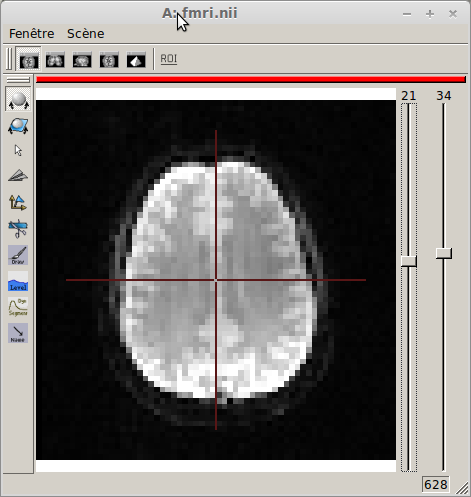
\includegraphics[width=0.7\textwidth]{fmri_anatomist}
\end{figure}

% Faire plein de figures pour montrer les observations...



\subsection{Segmentation}

\subsection{Zones d'activation}

\section{IRM de diffusion}

\subsection{Estimation des tenseurs}
La fonction \lstinline{Q2_IRMd.tenseur} utilise la méthode de la pseudo-inverse pour effectuer le calcul des tenseurs. Elle peut prendre en entrée un masque qui indique pour quels voxels calculer les tenseurs. Sont également mis à 0 tous les éléments de tenseurs qui:
\begin{enumerate}
\item Correspondent à un signal à $b=0$ nul.
\item Prennent une valeur NaN ou Inf. 
\end{enumerate}
La fig. \ref{tenseurs_fiber} illustre les tenseurs que nous avons ainsi obtenus sur une carte de FA (calculée grâce à l'alogrithme présenté dans la section suivante).
\begin{figure}
\begin{center}
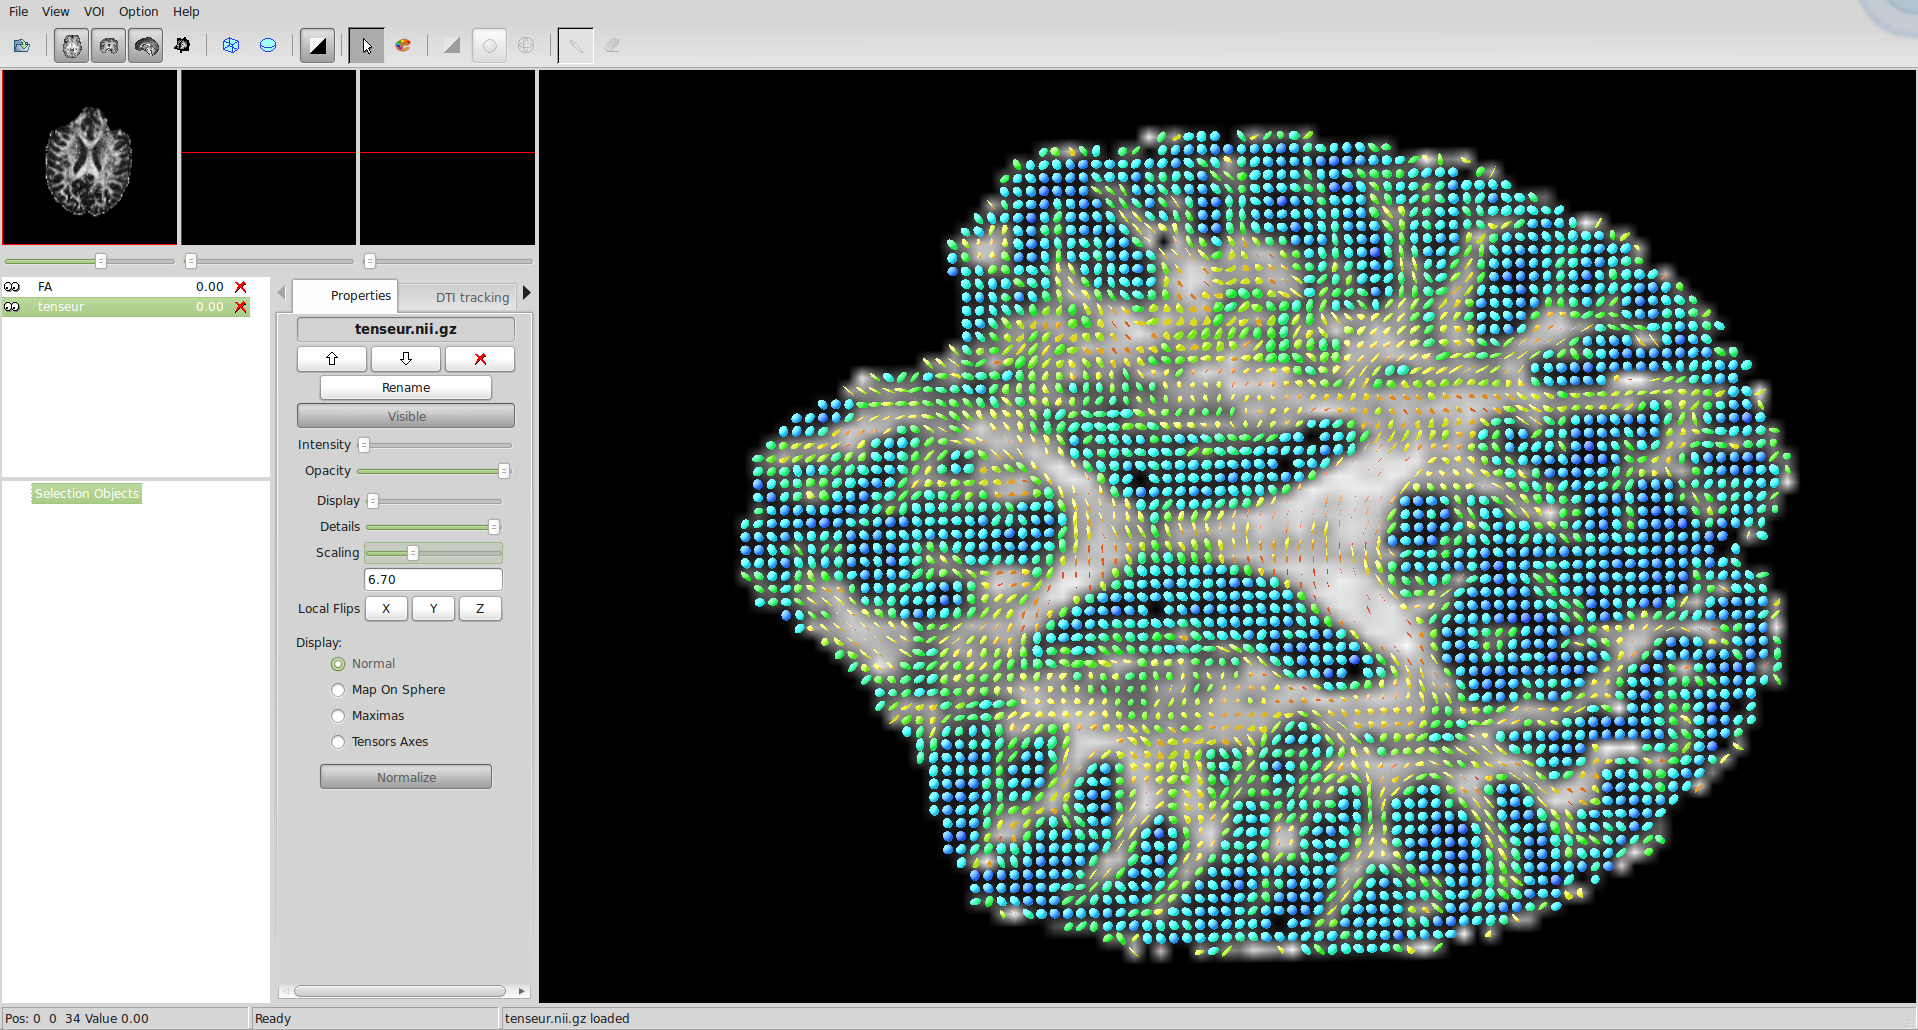
\includegraphics[scale=0.22]{tenseurs_fiber}
\caption{Illustration dans le Fibernavigator des tenseurs que nous avons obtenus grâce à la fonction \lstinline{Q2_IRMd.tenseur}. Les tenseurs sont superposés à la FA. À noter que seule une région identifiée comme étant le cerveau grâce à l'algorithme \lstinline{BET} de FSL est présentée. \label{tenseurs_fiber}}
\end{center}
\end{figure}

\subsection{FA et ADC}
La fonction \lstinline{Q2_IRMd.compAdcAndFa} calcule l'ADC et la FA à partir d'un champ de tenseur tel que calculé par la fonction \lstinline{Q2_IRMd.tenseur}. La fig. \ref{adc_fa} illustre pour certaines tranches l'ADC et la FA, respectivement. Les unités de l'ADC sont les mêmes que celles du coefficients de diffusion, soit $[longueur]^2/[temps]$, alors que la FA est sans unité.

\begin{figure}
\begin{center}
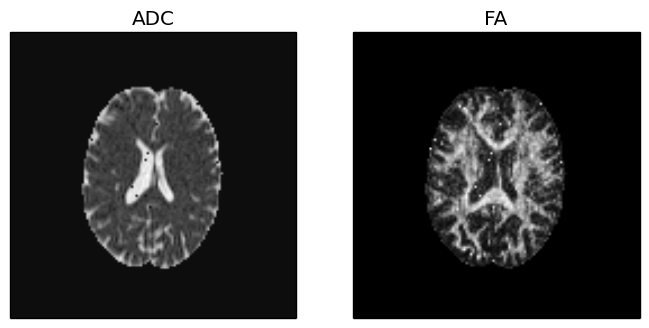
\includegraphics[scale=0.9]{adc_fa}
\caption{ADC et FA pour une tranche axiale du volume d'IRMd.\label{adc_fa}}
\end{center}
\end{figure}

\subsection{Tractographie}
La fonction \lstinline{Q2_IRMd.tracking} effectue une tractographie sur un champ de tenseurs. Lors de l'écriture de la fonction, nous avons remarqué

\section{Fusion}

\subsection{Justification}

\subsection{Connectivité des zones fonctionnelles}

\section{Bonus}

\subsection{FA et ADC}

\subsection{Tractographie avec Dipy}


\end{document}